% =============================
%  Imperial IRP – Title Page
% =============================
\documentclass[12pt,a4paper]{article}

% --------- page settings ----------
\usepackage{geometry}
\geometry{margin=2cm}
\usepackage{setspace}
\usepackage{url}
\usepackage{helvet}
\usepackage{enumitem} % For customizing lists
\usepackage{pgfgantt}
\usepackage{ragged2e}
\usepackage{float}
\usepackage{caption}
\usepackage{booktabs}
\usepackage{tabularx}
\usepackage{longtable}
\usepackage{array}
\usepackage[hidelinks]{hyperref}
\setcounter{tocdepth}{3}
\renewcommand{\familydefault}{\sfdefault}

\onehalfspacing
\setlength{\parskip}{0.5em}

\begin{document}
\begin{titlepage}
    \centering
    \vspace*{0cm}

    {\Large Imperial College London\par}
    \vspace{0.5cm}
    {\large Department of Earth Science and Engineering\par}
    \vspace{0.5cm}
    {\large MSc in Applied Computational Science and Engineering\par}

    \vspace{1.8cm}

    {\large Independent Research Project\par}
    {\large Final Report\par}

    \vspace{1.8cm}

    {\Large\bfseries
      Deep Learning in MRI K-space: A Novel Approach to Clinical Decision Support by Directly Learning Raw Signals\par}

    \vspace{1.5cm}

    {\large by\par}
    \vspace{0.0cm}
    {\Large Yiding Hao\par}

    \vspace{1.0cm}

    {\normalsize Email: \texttt{yiding.hao24@imperial.ac.uk}\par}
    {\normalsize GitHub username: acse-yh924\par}
    {\normalsize Repository: \url{https://github.com/ese-ada-lovelace-2024/irp-yh924.git}\par}

    \vspace{0.5cm}

    {\large Supervisors:\par}
    \vspace{0.0cm}
    {\normalsize Dr. Antony Sommerfeld\par}
    {\normalsize Dr. Tom Davison\par}
    {\normalsize Mr. Yassine Charouif\par}

    \vfill
    {\large August 2025\par}
\end{titlepage}



\newpage
\pagenumbering{roman}
\setstretch{0.9}
\tableofcontents

\section*{List of Abbreviations}
\vspace{2em}
\begingroup
\setlength{\tabcolsep}{14pt}
\renewcommand{\arraystretch}{2}
\noindent
\begin{tabularx}{\textwidth}{>{\bfseries}m{8cm} X}
ACS  & Autocalibration Signal \\
ASD  & Average Surface Distance \\
DCNN & Deep Convolutional Neural Network \\
FCN  & Fully Convolutional Network \\
GRU  & Gated Recurrent Unit \\
IFFT & Inverse Fast Fourier Transform \\
IFT  & Inverse Fourier Transform \\
LAX  & Long-Axis \\
MAE  & Mean Absolute Error \\
mIoU & mean intersection over union \\
MRI  & Magnetic Resonance Imaging \\
RNN  & Recurrent Neural Network \\
SAX  & Short-Axis \\
SVD  & Singular Value Decomposition \\
\end{tabularx}
\endgroup



\newpage
\clearpage
\pagenumbering{arabic}

\setstretch{1.25}
\section*{Abstract}
\addcontentsline{toc}{section}{Abstract}
AI assisted Magnetic Resonance Imaging (MRI) pipelines typically reconstruct images before analysis. However, unlike prior works such as AUTOMAP, this study investigates whether deep learning networks can bypass reconstruction and learn diagnostic features directly from raw K-space for downstream tasks. We propose a dual-axis SweepGRU encoder that scans K-space rows and columns to capture long-range dependencies, and a U-Net refiner for segmenting cardiac structures, together with auxiliary reconstruction and coarse-segmentation heads. We evaluate the effect of myocardial/cavity segmentation under full sampling and undersampling on CMRxRecon2023 cardiac MRI data. The proposed model obtains a mean Dice of 0.567 and a mean intersection over union (mIoU) of 0.505 on fully sampled data, indicating that frequency-domain representations contain diagnostically relevant features that can be extracted by proposed deep learning networks. Moreover, when supplied with a joint input of reconstructed images and K-space features, the model achieves better performance than with either modality alone, indicating the synergistic effect between the frequency and spatial domains. We further observe that under severe undersampling, the model with K-space input degrades significantly less than that with image input and performs better, offering a pathway to obtaining valuable information with shorter MRI scan time. These findings provide preliminary evidence that K-space can be used directly for downstream tasks and strengthen existing workflows. They also hold the potential to accelerate MRI acquisition, improve patient experience, and provide a methodological reference for sensor-level AI.

\newpage
\section{Introduction}

\subsection{Background}
MRI is an important medical imaging technology that has been widely applied in clinical diagnosis for its non-invasiveness, absence of ionizing radiation, and high soft-tissue contrast \cite{1}. The MRI image acquisition process involves two main steps: recording the original signal in the frequency domain space (K-space), and using methods such as Inverse Fourier Transform (IFT) to reconstruct images from K-space. Each sampling point in K-space encodes spatial frequency and phase information rather than direct image intensities that collectively determines the final image structure \cite{2}\cite{5}. The traditional MRI analysis process usually relies on reconstructed images as input, and then uses artificial features or deep learning models to perform tasks such as lesion segmentation, classification or detection \cite{3}.

The traditional "reconstruct before input" paradigm primarily focuses on spatial domain. However, the original K-space data comprises magnitude information that is equivalent to the image, and also contains phase and other features that may hold potential value \cite{4}. There are different methods to get K-space data. Cartesian scans sample k-space line-by-line and non-Cartesian scans sample continuous curved paths and thus require density compensation and gridding interpolation onto a Cartesian grid before fast Fourier transform \cite{6}. Under ideal conditions, K-space can be transformed through the IFT to almost losslessly reconstruct the image, but the way information is represented differs between the two domains. Therefore, directly analyzing K-space offers a new perspective for investigating the complementarity of different information domains in medical imaging tasks \cite{7}.


\subsection{Related Work}

In the field of medical imaging, MRI is widely used in the diagnosis and prognosis assessment of heart diseases since it can provide high-resolution information on the structure and function of the heart \cite{8}. In recent years, deep learning methods have made remarkable progress in multiple aspects in MRI analysis.

In the domain of reconstruction, end-to-end deep networks such as E2E-VarNet use learnable image-domain regularizers and refine K-space via data-consistency steps. Evaluations on large-scale benchmark datasets such as fastMRI illustrate that these methods have improved the accuracy and speed of undersampled MRI reconstruction, providing a viable path for faster image acquisition \cite{9}. Beyond image reconstruction, machine learning has also improved downstream tasks such as lesion segmentation and classification. Using population data from the UK Biobank cine-CMR, Bai et al. developed a Fully Convolutional Network (FCN) for automated cardiac structure segmentation. From the resulting segmentation masks, the researchers calculated ejection fraction, cardiac chamber volume, and other functional indices, thereby establishing a feasible pipeline from segmentation to functional quantification and disease analysis \cite{10}. In classification tasks, deep models of multimodal MRI fusion have been used for tasks such as Alzheimer's disease staging and brain tumour grading \cite{28}. Li et al. developed a Deep Convolutional Neural Network (DCNN) on multi parametric MRI to perform molecular subtyping of gliomas, achieving performance superior to traditional radiomics methods \cite{11}.

In contrast, research of applying deep learning directly to MRI K-space is relatively new. K-space data is primarily used for image reconstruction. Zhu et al. proposed the AUTOMAP framework, which directly maps K-space to images via the deep network, achieving performance comparable to or even superior to traditional reconstruction methods \cite{12}. Oh et al. proposed ETER-net, which uses a bidirectional recurrent neural network to directly map multi-channel K-space data to the image domain and combines CNN to refine the reconstruction results. This network effectively eliminates artifacts and can support multiple sampling trajectories. Compared to AUTOMAP, it has fewer parameters and higher resolution, and further improves detail and structural fidelity by introducing adversarial and perceptual losses \cite{13}. In addition, researchers have begun to explore the direct use of K-space data for diagnosis-related tasks. For example, Ravishankar et al. performed brain structure segmentation and classification directly from K-space using deep neural networks, achieving accuracy comparable to image-domain methods \cite{14}. Bian et al. proposed a dual-path attention fusion network, in which one path processes K-space to extract global frequency-domain features, and the other path processes images to capture local details, with the two fused via an attention mechanism, thereby improving performance in brain tumor segmentation tasks \cite{15}.

These studies indicate that there is complementarity in the expression of information between frequency-domain and image-domain features. K-space may provide additional global information for deep models, while images presents the local structure more intuitively. Therefore, in-depth investigation into how to effectively extract K-space information and employ it to complement image-based models holds the potential to become one of the key directions in MRI deep learning research.


\subsection{Research Aims and Significance}

\subsubsection{Research Aims}
This research work investigates if deep learning models can extract diagnostic features directly from raw MRI signals, bypassing the conventional image reconstruction step. For this purpose, we aim to design and evaluate models capable of analysing complex high-dimensional frequency-domain data and correlate them with pathological findings, thereby enabling a deeper understanding of how K-space can be exploited by deep learning for medical diagnosis.

The specific objectives of this research work can be divided into following points:
\begin{enumerate}
\item Investigate if the K-space, which is difficult for humans to understand, can provide diagnostically relevant features through deep learning models such as CNN or Recurrent Neural Network (RNN) encoders. This involves using deep learning models for self-supervised reconstruction, applying K-space-based models directly for end-to-end segmentation tasks, and evaluating the models by examining loss curves and other performance metrics. The success is defined as achieving a Dice score more than 0.5.
\item Examine if K-space can provide effective complementary features to image-based models. This could be achieved by extracting features from both K-space and images, and verifying whether the architecture can outperform models based on single modality or not.
\item Explore additional benefits that K-space-based models could bring to current medical imaging pipelines, such as faster data acquisition times and better patient experience. Success if K-space-based model shows less performance degradation than the image-based model under undersampling.
\end{enumerate}

\subsubsection{Research Significance}
This research work expands the traditional MRI AI analysis paradigm to the field of raw machine data and local sensors, and provides insights for future AI systems that integrate raw signal data into clinical workflows. It validates the feasibility of using deep learning models to extract frequency-domain features, the complementarity of frequency-domain and image-domain features, and the advantages of frequency-domain methods when using undersampled data. These observations contribute to further improving the performance of current pipelines by fusing the image domain with the frequency domain, and have the potential to accelerate the MRI scan and improve the patient experience.



\section{Methodology}
We first assessed the feasibility of the proposed network, then evaluated its performance and compared different input schemes. Finally, we explored its application potential on undersampled data. This section will introduce the datasets, architecture details, and training strategy.

\subsection{Dataset}
\subsubsection{Data Gathering}
To evaluate the proposed approach, we employed two publicly available MRI datasets: fastMRI and CMRxRecon2023.

The fastMRI dataset is jointly released by NYU Langone and Facebook AI Research, and aims to accelerate MRI reconstruction using AI. This dataset is acquired using 1.5T and 3T MRI scanners, including thousands of de-identified raw K-space acquisitions, with approximately 1,500 knee MRI scans, about 6,970 brain MRI scans, as well as hundreds of prostate and breast MRI scans \cite{16}\cite{17}.

CMRxRecon2023 is derived from the Medical Image Computing and Computer Assisted Intervention (MICCAI) 2023 "Cardiac MRI Reconstruction Challenge", providing a large-scale, multi-contrast, and multi-view K-space dataset of cardiac MRI. The data cover cine sequences and T1/T2 mapping, which are acquired from 300 healthy volunteers. The data are collected using a 3T Siemens MAGNETOM Vida scanner and 32-channel cardiac coils, including short-axis (SAX) and long-axis (LAX) perspectives, with Autocalibration Signal (ACS), which represents fully sampled low-frequency k-space lines at the center. Some of the data are accompanied by manual segmentation labels for cardiac cavities and myocardial structures, which were annotated by radiologists with over five years of experience in cardiac imaging \cite{18}. These masks and their corresponding images are stored in NIFTI format. Figure 1 shows the K-space, reconstructed image and its segmentation label of a certain frame.


\begin{figure}[H]
    \centering
    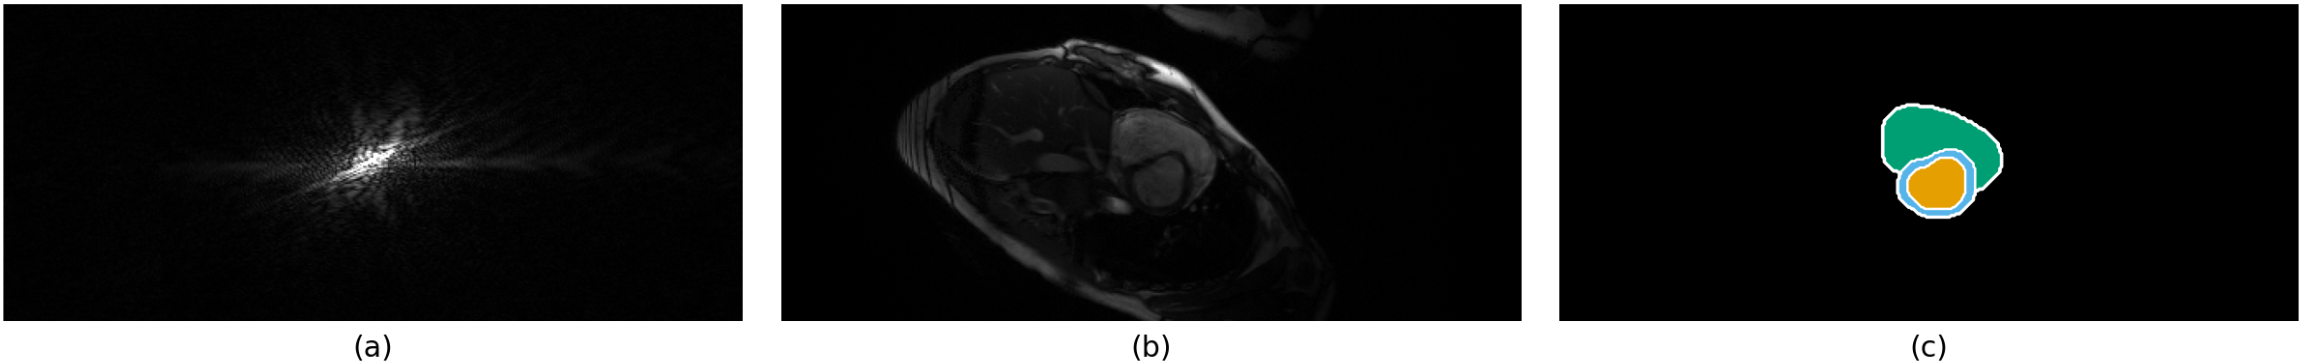
\includegraphics[width=1.0\linewidth]{report_image/dataset_visualise.png}
    \captionsetup{width=.9\linewidth}
    \caption{Example frame from a short-axis cardiac MRI sequence: (a) K-space magnitude visualization in logarithmic scale; (b) corresponding image reconstructed via IFFT; (c) segmentation label (including left ventricle, left ventricular myocardium, and right ventricle).}
\end{figure}

All datasets are stored in MATLAB ".mat" format, containing the number of temporal frames, coil channels, and the original sampling points along the kx and ky directions. In this research work, we used a subset of brain images for image reconstruction to assess whether deep learning networks can extract meaningful information from K-space. We also employed the SAX data from the CMRxRecon2023 validation set for the automatic segmentation of cardiac cavities and myocardial structures.


\subsubsection{K-space Introduction}

In MRI, K-space data are obtained by applying a series of radio frequency pulses and magnetic field gradients under an external magnetic field and collecting signals in a spatially encoded sequence, and each point encodes a specific spatial frequency component of the image. The complete K-space contains all spatial-frequency information, and combining these frequencies via an IFT yields the full image in the spatial domain. This process is usually achieved by applying the two-dimensional Inverse Fast Fourier transform (IFFT) to the data from each coil channel respectively. Figure 2 illustrates how a single data point in K-space affects the entire image. The central regions of K-space contain low spatial frequencies, corresponding to coarse anatomical structures, while the peripheral regions encode high spatial frequencies, capturing fine details and sharp edges. Since many disease biomarkers may be reflected in both coarse structures and fine spatial details, magnitude and phase information in K-space are both related to disease detection. The orientation of the patterns reflects the direction of spatial variation in the image \cite{2}\cite{19}.

\begin{figure}[H]
    \centering
    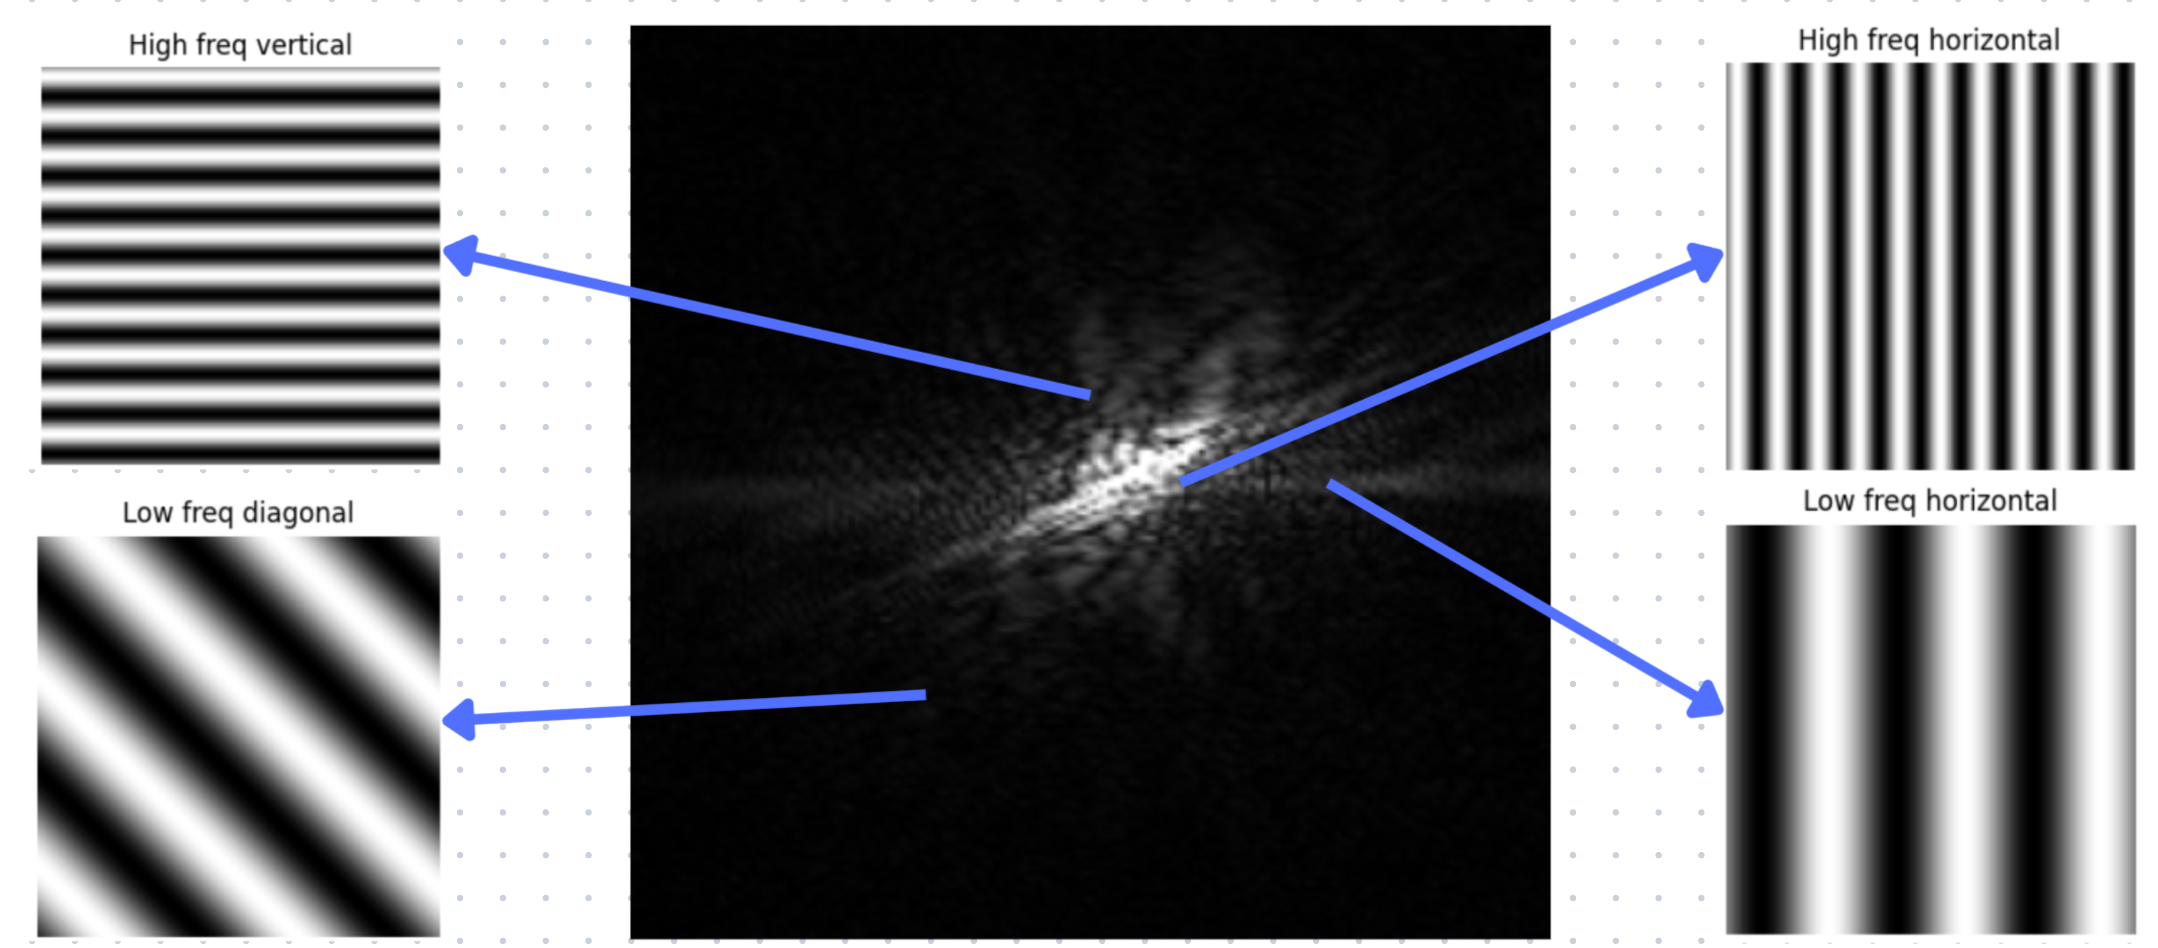
\includegraphics[width=0.8\linewidth]{report_image/k_visualise.png}
    \captionsetup{width=.75\linewidth}
    \caption{K-space to image mapping: frequency magnitude and orientation correspondence}
\end{figure}

\begin{equation}
\mathcal{F}[f(t)] = \int_{-\infty}^{+\infty} f(t) e^{-i \omega t} \, dt = F(\omega)
\end{equation}

\begin{equation}
\mathcal{F}^{-1}[F(\omega)] = \frac{1}{2\pi} \int_{-\infty}^{+\infty} F(\omega) e^{i \omega t} \, d\omega = f(t)
\end{equation}

The IFT mathematically converts the spatial frequency components stored in K-space into the spatial domain pixel intensities. Equations 1 and 2 define the Fourier transform and IFT. In the context of MRI, \( f(t) \) corresponds to the image-domain signal, and \( F(\omega) \) corresponds to the K-space data. The exponential terms describe the decomposition and reconstruction of the signal into and from sinusoidal basis functions, respectively \cite{2}.


\subsection{Data Preprocessing}

\subsubsection{General Preprocessing}
MR signals are radiofrequency waves that contain amplitude and phase information, so the raw K-space data are stored in complex form \cite{2}. We converted them into PyTorch complex tensors and separated the real and imaginary parts into two channels so that the deep learning model can handle it directly. Since the K-space data in the dataset vary in size, we performed center cropping and zero-padding in the frequency domain to unify them to the target resolution. For the fastMRI dataset, the target size was (320, 640); for the CMRxRecon dataset, the target was (192, 448). During cropping or padding, the center of the frequency domain was preserved to avoid affecting the reconstruction of the image.

\begin{equation}
k^{(v)}(h,w) = \sum_{c=1}^{C} a_{v,c}\, k_c(h,w), \qquad v=1,\ldots,N_v 
\end{equation}

The CMRxRecon data used in this research work are single-coil, while the fastMRI data are multi-coil, and the number of coils is not unique. We applied singular value decomposition (SVD) based coil compression method, which factorizes the coil dimension into orthogonal components, and retained four virtual coils. This reduced variability in coil configuration while preserving most of the signal energy \cite{20}. Equation 3 shows this calculation process, where \(a_{v,c}\) represents the projection weight from the SVD basis, \(C\) represents the number of original coils, and \(N_v\) represents the number of virtual coils retained (in our experiments, \(N_v=4\)).

Moreover, because each case contains multiple frames, we split the dataset at the case level using the case ID. This will guarantee that the training set and the validation set do not contain similar data, preventing the data leakage.


\subsubsection{Undersampling}
To investigate if deep learning models can extract features from undersampled K-space data, we applied one-dimensional variable density Cartesian undersampling along the phase-encoding direction while keeping the frequency-encoding direction fully sampled. The sampling mask retained a small continuous low-frequency area at the center of the K-space as ACS lines. We employed an acceleration factor of 24, which controlled the ratio between the total number of phase-encoding lines in the fully sampled field and the number of lines preserved. In Cartesian undersampling, the retained lines were randomly selected according to a variable-density probability distribution outside the ACS region, resulting in denser sampling in the central region and sparser sampling in the peripheral high-frequency region \cite{21}.

\begin{figure}[H]
    \centering
    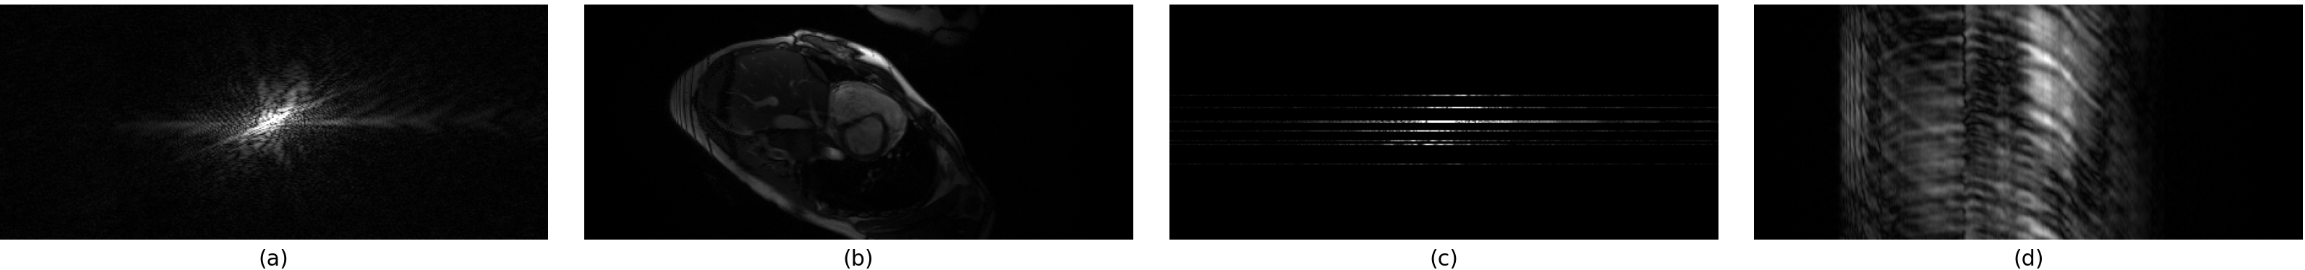
\includegraphics[width=1\linewidth]{report_image/under-sampling_visualise.png}
    \captionsetup{width=.9\linewidth}
    \caption{Fully sampled vs. undersampled K-space and corresponding reconstructions: (a) fully sampled K-space; (b) IFFT reconstructed image from (a); (c) Cartesian undersampled K-space; (d) IFFT reconstructed image from (c).}
\end{figure}

Figure 3 illustrates the original K-space, its undersampled counterpart, and the corresponding reconstructed images. It shows that undersampling degrades the structural clarity of the reconstructed image, posing a challenge for deep learning models to analyse these data.


\vspace{-0.5em}
\subsubsection{Data Augmentation}
\vspace{-0.5em}
K-space is frequency-domain data, traditional image enhancement methods might destroy its structure and feature. Therefore, we employed specific frequency-domain data augmentation methods in the reconstruction task, including global phase shift, linear phase ramp and horizontal or vertical flip. Table 1 shows the details and purposes of these methods. In this study, data augmentation was only used in the reconstruction experiment because corresponding segmentation labels are difficult to go through the same K-space augmentation operations.


\begin{table}[H]
\centering
\caption{K-space augmentation methods}
\renewcommand{\arraystretch}{1.15}
\begin{tabularx}{\linewidth}{@{} lXXX @{}}
\toprule
\textbf{Augmentation} &
\textbf{K-space Operation} &
\textbf{Purpose} \\
\midrule
\textbf{Global phase shift} &
Multiply K-space samples by a constant complex phase factor &
Increase phase invariance \\
\textbf{Linear phase ramp} &
Apply a coil-wise linear phase gradient along kx and/or ky &
Simulate motion or slice misalignment \\
\textbf{Horizontal / vertical flip} &
Flip K-space along frequency-encoding or phase-encoding direction &
Increase orientation diversity \\
\bottomrule
\end{tabularx}
\end{table}

\vspace{-2em}
\subsection{Model Architecture}
\vspace{-1em}
In this research work, multiple architectures were implemented and compared. Each point in K-space is relative to the whole reconstructed image, thereby it is difficult to extract effective features using normal CNNs. Therefore, we explored several architectures that are able to capture global information, including complex-CNN, Transformer, and RNN. Ultimately, inspired by ETER-net, we designed an architecture that is suitable for K-space input \cite{13}. The overall architectural details are shown in Figure 4.
\vspace{1em}

\begin{figure}[H]
    \centering
    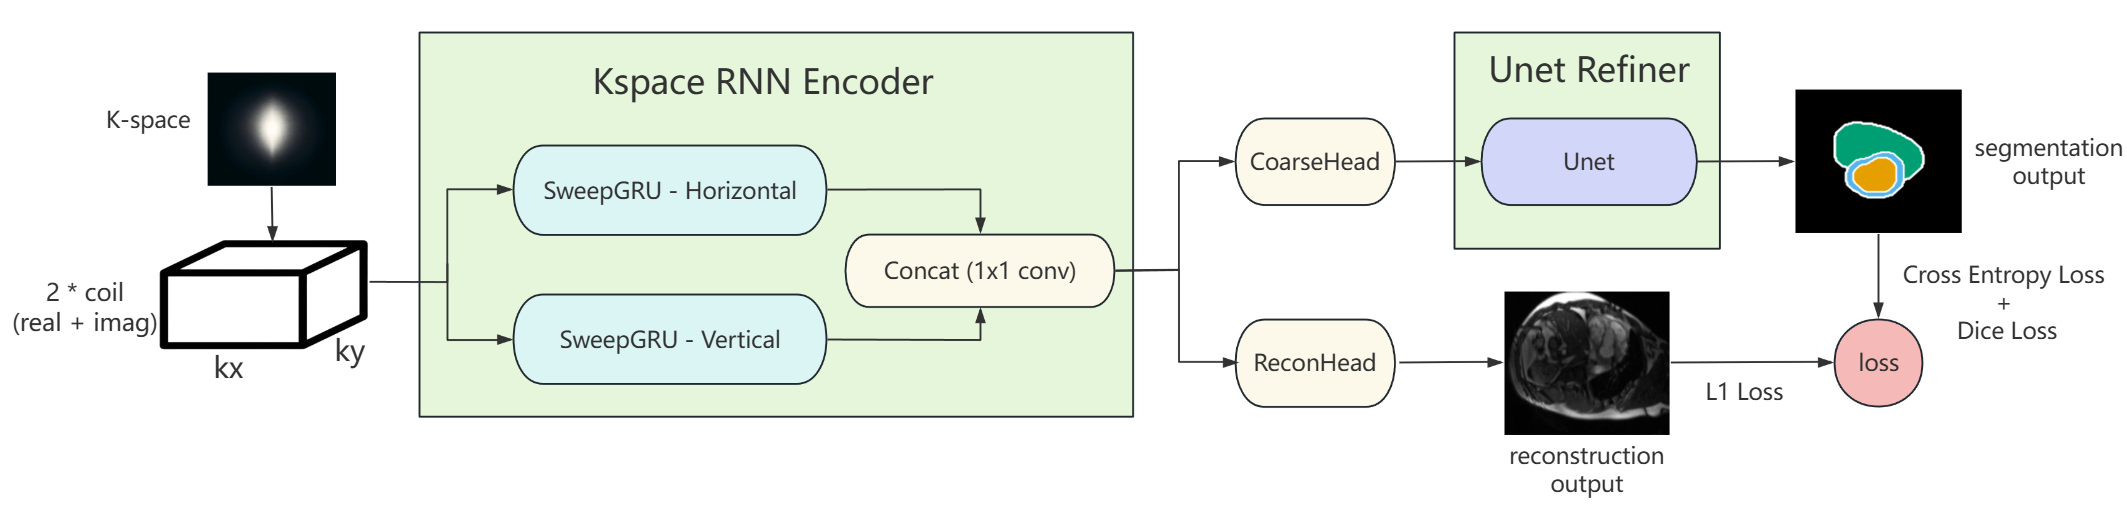
\includegraphics[width=1\linewidth]{report_image/seg_process.png}
    \captionsetup{width=.9\linewidth}
    \caption{Proposed deep learning framework for segmentation of cardiac chambers and myocardium directly from raw K-space.}
\end{figure}


\subsubsection{Framework Details}

\noindent \textbf{(1) K-space RNN Encoder}

The encoder consists of two SweepGRU modules, which are recurrent feature extractors specialized for sequential traversal of 2D K-space data along a certain axis. Different from a single layer Gated Recurrent Unit (GRU), SweepGRU stacks multiple bidirectional GRU layers, and each layer receives the concatenated forward and backward hidden states from the previous layer so as to achieve richer contextual encoding \cite{22}. Residual connections are applied between GRU layers to enhance training stability \cite{23}. After sequentially traversing K-space lines in both orientations, the outputs from the two encoders are fused by a 1x1 convolution to yield a unified representation.

The encoder is able to capture the global structural relationships in the frequency domain by sequentially traversing K-space in both orientations. It is able to effectively extract features for subsequent image reconstruction and segmentation tasks.


\noindent \textbf{(2) Coarse Segmentation Head}

The encoded K-space features are input to a lightweight coarse segmentation head, which is composed of two convolutional layers. The CoarseHead converts frequency-domain features to a rough spatial domain mask, so that the U-Net refiner can focus on boundary refinement and detail enhancement rather than learning from scratch. In addition, this structure can serve as a bridge between the frequency domain and the spatial domain, making the features learned by K-space RNN encoder easier to be used by subsequent spatial domain modules.


\noindent \textbf{(3) Reconstruction Head}

The reconstruction head aims to predict the magnitude image using the features provided by the K-space RNN encoder. The lightweight module consists of two convolutional layers, a 3×3 convolution with ReLU activation to reduce the channel dimension followed by another 3×3 convolution to produce a single-channel output. 

This module is to verify if the encoder can extract meaningful information and regularize the architecture and encourage it to preserve spatially coherent information. In the segmentation task, the encoder tends to learn features directly related to segmentation. Without auxiliary constraints, the model might overlook the information related to the original signal structure, thereby increasing the risk of overfitting. The reconstruction task will force the model to retain more complete frequency-domain information, thereby making the features more general and stable.


\noindent \textbf{(4) U-Net Refiner}

We introduced a standard U-Net architecture after the coarse segmentation head to complete the refined segmentation. The U-Net refiner takes the coarse segmentation result as input and outputs the final result. It is composed of multiple convolutional and max-pooling blocks, which gradually extract high-level semantic features. Following the encoder, a convolutional block with a higher number of channels is employed in the bottleneck layer for global context integration and feature compression. The decoder is composed of several upsampling modules, and each of them includes bilinear interpolation upsampling and convolutional blocks. Skip connections transfer features directly from upsampling modules to corresponding downsampling modules to mitigate feature degradation and retain details of the low-level features. After the standard U-Net architecture, the feature map is mapped to the category dimension through a 1×1 convolution.

\subsubsection{Fusing K-space and Reconstructed Images as Inputs}
We further compared two alternative input configurations: only using the image reconstructed by IFFT, and using the combination of IFFT reconstructed image and K-space. The network structure was also adjusted accordingly. For the case of using only the image as input, the reconstructed image was directly fed into the U-Net refiner. For the case of combining image and K-space as input, the IFFT-reconstructed image was fused with the output of the coarse segmentation head using channel-wise gating and pixel attention before being fed into the U-Net refiner. In both cases, we removed the reconstruction head and focused only on the final segmentation results. Figure 5 illustrates the updated network structure that uses the combined input.

\begin{figure}[H]
    \centering
    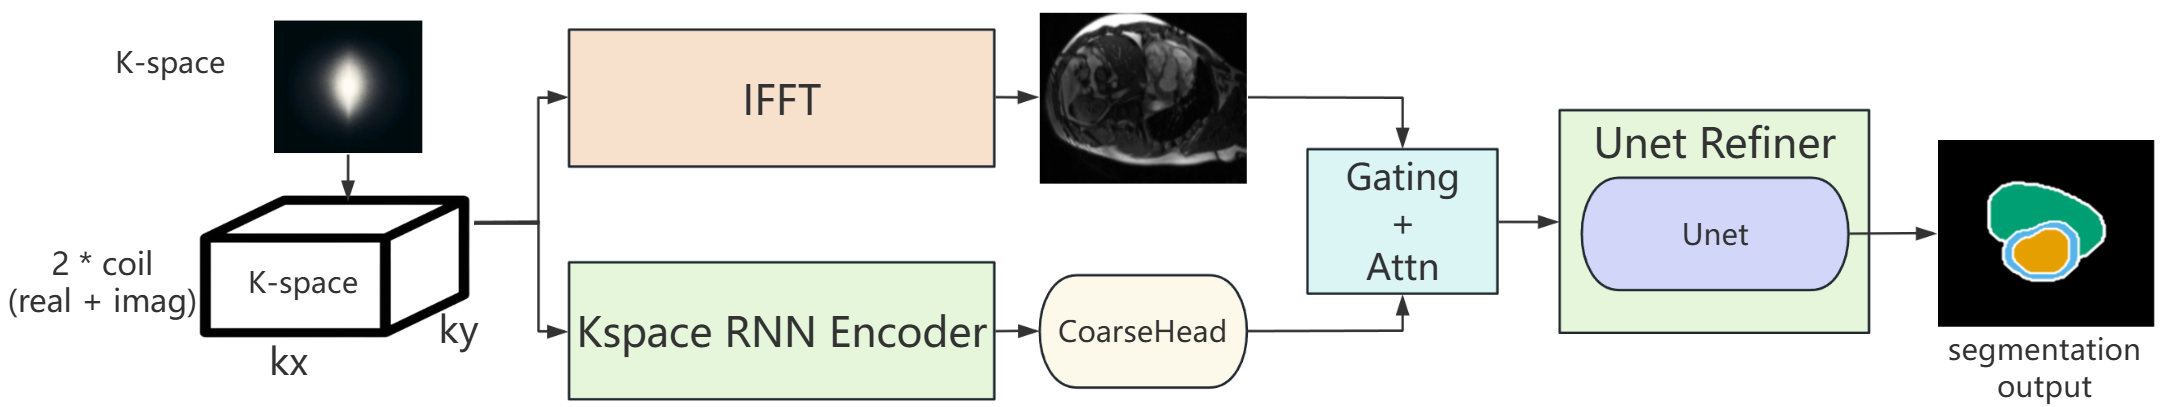
\includegraphics[width=1\linewidth]{report_image/dual_process.png}
    \captionsetup{width=.9\linewidth}
    \caption{Updated network structure taking fused K-space and reconstructed images as inputs}
\end{figure}


\subsection{Training Strategy}
For the reconstruction experiment, the model adopts Mean Absolute Error (MAE) as the loss function, to encourage sparsity in the residuals. MAE loss is less sensitive to outliers, so it is particularly beneficial for preserving structural details \cite{24}.

In the segmentation task, the network is trained under the multi-task learning paradigm, and the overall loss function consists of three parts. The first part is the same as the loss function used in the reconstruction task, derived from the reconstruction head. The other two components are cross-entropy loss and Dice loss. Cross-entropy measures the difference between the output and the label. The Dice loss measures the degree of overlap between the predicted results and the label, focusing on the ratio of correctly segmented pixels instead of its absolute number. It is effective in handling class imbalance situations, and is able to improve the segmentation performance for minority classes \cite{25}. The final loss is shown in Formula 3. Since the reconstruction loss is relatively small compared to other loss terms, we applied a scaling factor of 3 to balance its contribution based on hyperparameter tuning.


\vspace{-0.5em}
\section{Results}
\vspace{-1em}
We evaluated the proposed network in three scenarios and compared its performance under different input schemes.

\vspace{-0.5em}
\subsection{Sanity Check: Simple Reconstruction from K-space}

In the reconstruction task, MAE is evaluated to check the feasibility of this architecture. Figure 6 shows the MAE reconstruction loss of every training epochs.

\begin{figure}[H]
    \centering
    
\includegraphics[width=0.7\linewidth]{report_image/curve_recon.png}
    \captionsetup{width=.9\linewidth}
    \caption{Reconstruction MAE during training}
\end{figure}


\subsection{Segmentation on Fully Sampled K-space}
A variety of metrics were used to evaluate the segmentation performance of the model, including pixel accuracy, cross-entropy, mIoU, and mean Dice. Pixel accuracy measures the proportion of correctly classified pixels; mIoU and mean Dice measure the overlap between the prediction and the label. The mIoU calculates the intersection over union of each category separately before taking the average, while mean Dice gives higher weights to the overlapping areas, so it is more sensitive to small targets \cite{26}. These metrics cover two major aspects including classification accuracy and region overlap. However, for medical image segmentation, clinically relevant metrics are also of great importance. Therefore, we introduced the Average Surface Distance (ASD), which evaluates the average distance between the predicted and ground truth contours, to obtain stronger clinical interpretability \cite{27}. Moreover, we calculated the Cohen's\_dz, which quantifies the magnitude of the average improvement relative to inter-patient variability to show the statistical significance of the performance difference between the K-space model and image model. Table 2 and 3 present the model’s results on the validation set and the corresponding confusion matrix. 

% \vspace{1em}
\begin{table*}[h]
\centering
\begin{minipage}{0.48\textwidth}
    \centering
    \caption{Results of the proposed model on validation set}
    \label{tab:val_results}
    \renewcommand{\arraystretch}{1.15}
    \begin{tabularx}{\linewidth}{@{} l >{\raggedleft\arraybackslash}X @{}}
        \toprule
        \textbf{Metric} & \textbf{Value} \\
        \midrule
        Pixel Accuracy & 0.9819 \\
        Cross Entropy & 0.072 \\
        Mean Dice    & 0.5674 \\
        Mean IoU    & 0.505 \\
        Overall ASD & 4.325 \\
        \bottomrule
    \end{tabularx}
\end{minipage}\hfill
\begin{minipage}{0.45\textwidth}
    \centering
    \captionsetup{width=.9\linewidth}
    \caption{Pixel-based confusion matrix on the validation set}
    \label{tab:cm_val}
    \renewcommand{\arraystretch}{1.15}
    \scriptsize
    \setlength{\tabcolsep}{4pt}
    \resizebox{\linewidth}{!}{%
    \begin{tabular}{@{} r r r r r @{}}
    \toprule
    \textbf{} & \textbf{0} & \textbf{1} & \textbf{2} & \textbf{3} \\
    \midrule
    0 & 10095681 & 19456 & 34843 & 31240 \\
    1 & 7451     & 46502 & 16784 & 636  \\
    2 & 20693    & 10092 & 28366 & 5086  \\
    3 & 35977    & 573   & 5588  & 48968 \\
    \bottomrule
    \end{tabular}}

\end{minipage}
\end{table*}


\noindent \textbf{Comparison with Image and Hybrid Inputs}

In order to compare the effectiveness of our proposed method with the conventional image-based approach, we evaluated the model that takes K-space inputs against a model that takes IFFT-reconstructed image input. Subsequently, we fused the features extracted by the K-space RNN encoder with the reconstructed image and fed them together into the U-Net refiner. Figure 5 illustrates the prediction results of the three models in several cases, and Table 4 provides a detailed quantitative comparison of their performance. 



\begin{table}[h]
\centering
\caption{Segmentation performance comparison on fully sampled data.}
\label{tab:tab4}
\setlength{\tabcolsep}{6pt}
\begin{tabular*}{0.95\linewidth}{@{\extracolsep{\fill}} lccccc}
\toprule
Model & Pixel Acc & Mean Dice & mIoU & ASD \\
\midrule
K-space only      & 0.9819 & 0.5674 & 0.505 & 4.325 \\
image only  & 0.994 & \textbf{0.8074} & 0.7639 & 1.427 \\
K-space + image   & \textbf{0.9943} & 0.8012 & \textbf{0.7736} & \textbf{1.2212} \\
\midrule
Effect size (Cohen's $d_{\mathrm{z}}$, K-space vs. Image) & \multicolumn{4}{c}{1.30} \\
\bottomrule
\end{tabular*}
\end{table}



\begin{figure}[H]
    \centering
    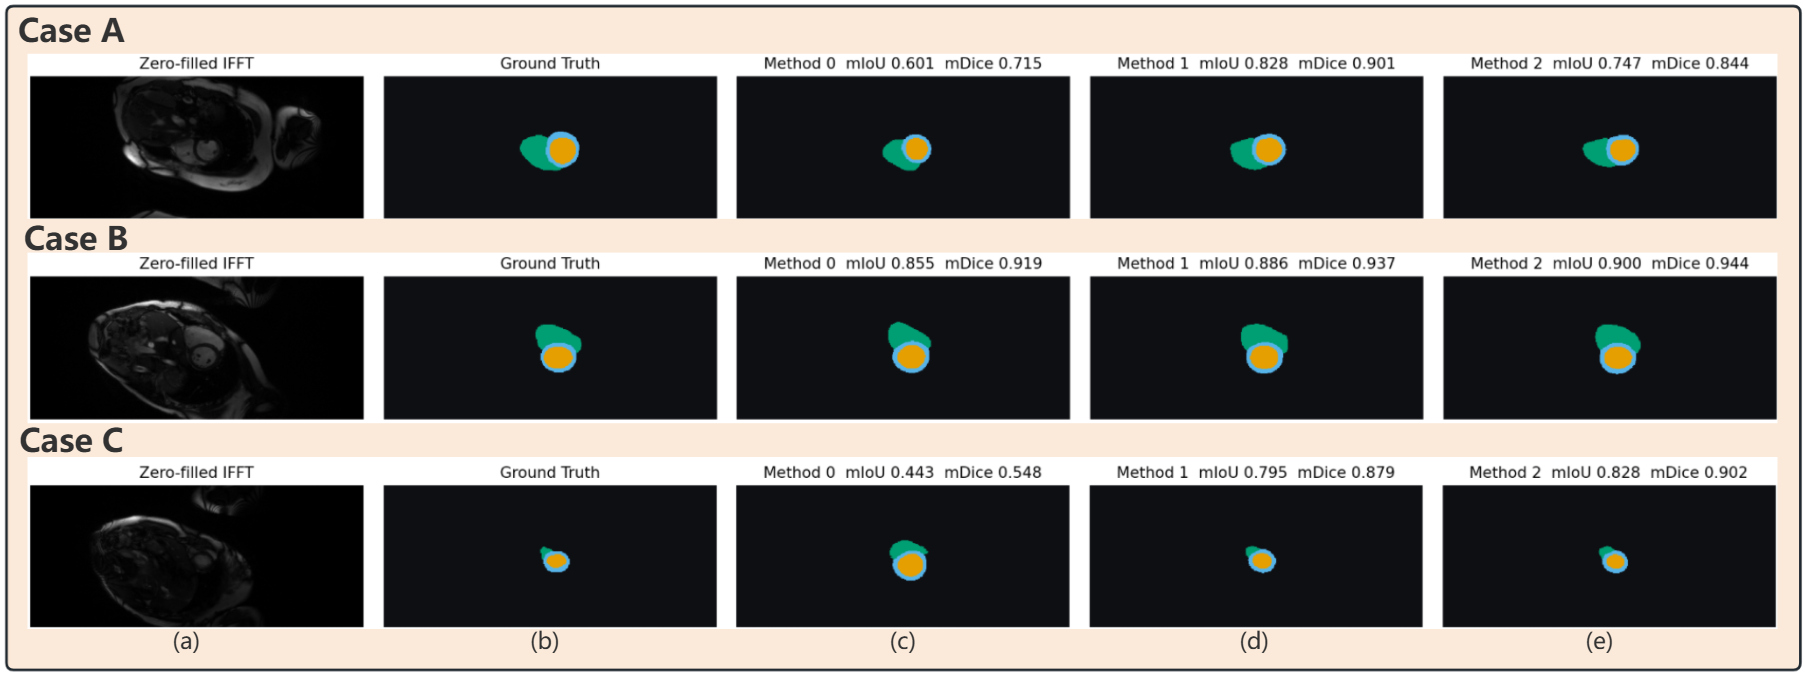
\includegraphics[width=1.0\linewidth]{report_image/full_compare.png}
    \captionsetup{width=.9\linewidth}
    \caption{Comparison of cardiac MRI segmentation on fully sampled data. (a) zero-filled IFFT; (b) ground truth; (c) K-space input; (d) image input; (e) hybrid input.}
\end{figure}


\subsection{Segmentation on Undersampled K-space}
We also trained and evaluated the network with severely undersampled K-space data to examine its performance under accelerated MRI acquisition. Figure 8 and Table 5 present the model performance on aggressively undersampled data with an acceleration factor of 24.


\begin{table}[h]
\centering
\caption{Segmentation performance comparison on undersampled data.}
\label{tab:tab4}
\setlength{\tabcolsep}{6pt}
\begin{tabular*}{0.95\linewidth}{@{\extracolsep{\fill}} lccccc}
\toprule
Model & Pixel Acc &  Mean Dice & mIoU & ASD \\
\midrule
K-space only      & 0.975  & 0.5077 & 0.4412 & 5.677 \\
image only        & 0.975  & 0.4789 & 0.4238 & 7.017 \\
K-space + image   & \textbf{0.9784} & \textbf{0.5401} & \textbf{0.4794} & \textbf{5.1071} \\
\midrule
Effect size (Cohen's $d_{\mathrm{z}}$, K-space vs. Image) & \multicolumn{4}{c}{0.20} \\
\bottomrule
\end{tabular*}
\end{table}


\begin{figure}[H]
    \centering
    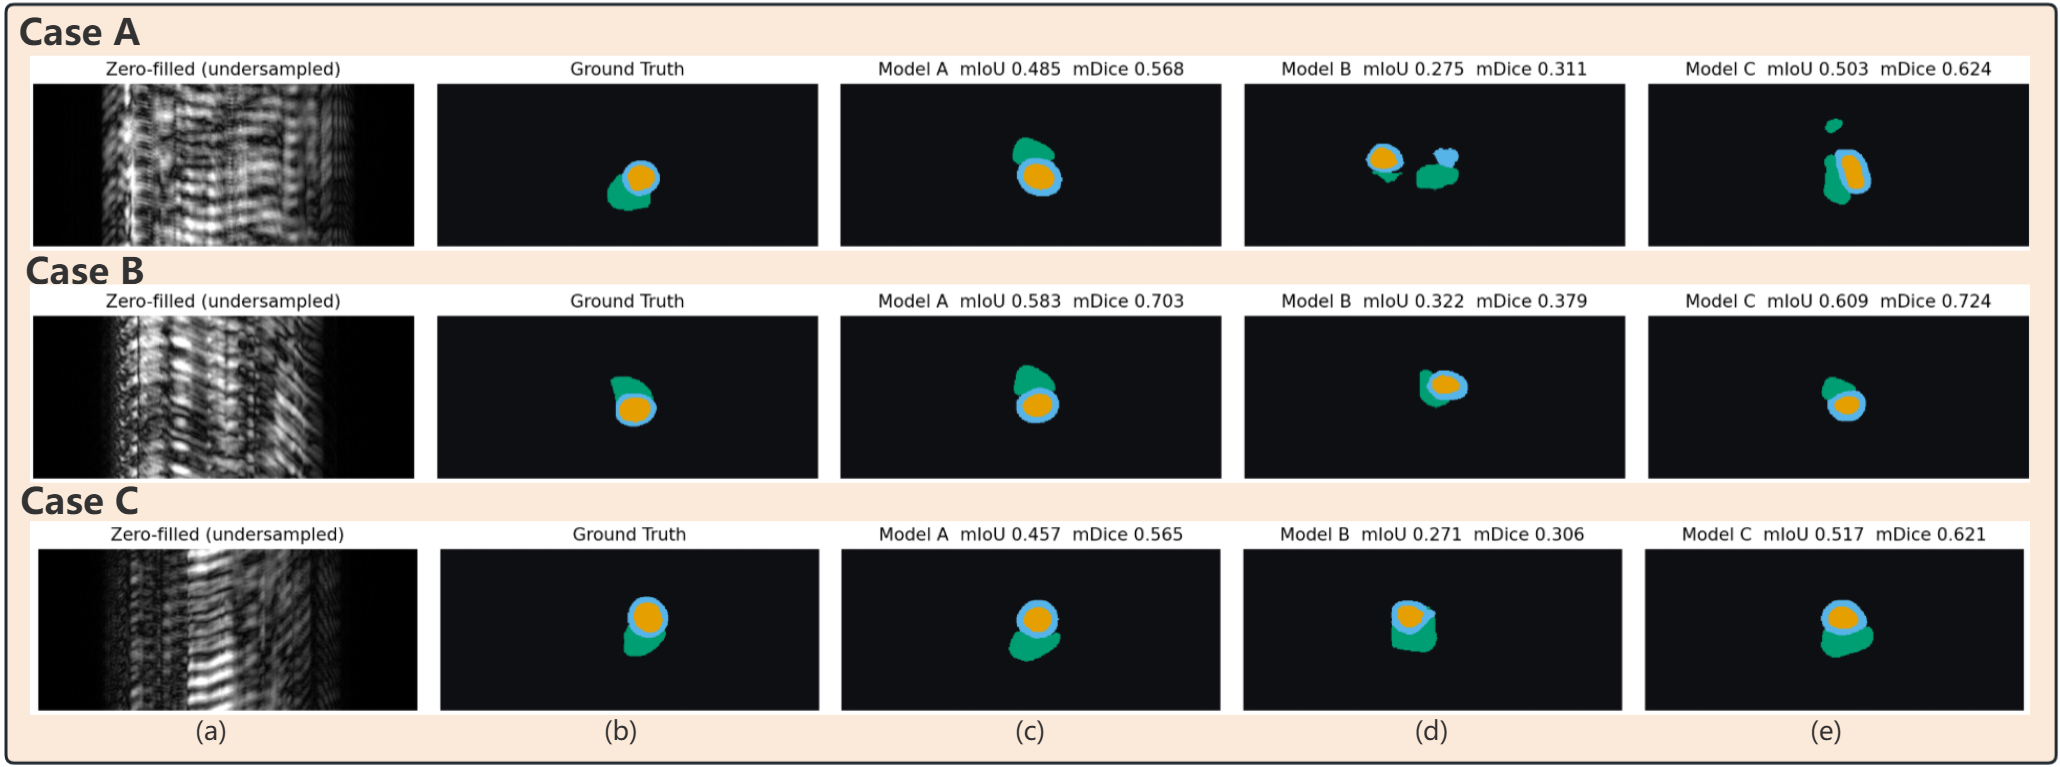
\includegraphics[width=1.0\linewidth]{report_image/under_compare.png}
    \captionsetup{width=.9\linewidth}
    \caption{Comparison of cardiac MRI segmentation on undersampled data. (a) zero-filled IFFT; (b) ground truth; (c) K-space input; (d) image input; (e) hybrid input.}
\end{figure}



\section{Discussion}
\vspace{-0.5em}
This research work explores the feasibility of employing deep learning to extract effective features directly in the frequency domain (K-space) and use them for downstream tasks. We focused on designing a framework with global perception to align with the physical properties of the frequency domain. Drawing inspiration from the ETER-net, we introduced several structural adjustments to design an end-to-end framework capable of segmenting directly from K-space, which utilises an RNN to sequentially scan the K-space.

We first assessed if the coarse segmentation head can provide a gradually refined result to vindicate that the feature extractor is able to extract meaningful features of K-space to a certain degree. Subsequently, we evaluated the segmentation performance using fully sampled K-space and compared the results across different input types. To further investigate the model's capability to provide effective predictions from undersampled K-space, we conducted an additional set of experiments and compared their performance.

\vspace{-1em}
\subsection{Interpretation of Simple Reconstruction from K-space}
\vspace{-0.5em}
In the reconstruction task, the objective of this research work is not to obtain the reconstructed image, as it can be obtained directly through IFFT, but to preliminarily determine if the K-space RNN encoder could provide enough information for the subsequent network. Therefore, the network employs a simple reconstruction head to ensure the efficiency of the overall network. This design enables rapid verification of the experimental feasibility and is able to provide the reconstruction loss in the segmentation task without significantly compromising the model's efficiency.

Figure 6 illustrates that the MAE reconstruction loss decreases steadily during training, which indicates that the K-space encoder can learn globally consistent features even with a lightweight reconstruction head.


\vspace{-1em}
\subsection{Interpretation of Fully Sampled K-space Segmentation}
\vspace{-0.5em}
As shown in Table 2 and Table 3, the proposed framework achieved a pixel accuracy of 0.982, indicating that most pixels are correctly classified. In terms of overlap-based metrics, the model obtained a mean Dice score of 0.567 and an mIoU of 0.505, reflecting that the prediction results have a certain degree of region-level consistency with the ground truth. To further evaluate boundary accuracy, we calculated the ASD, and the ASD of all categories reached 4.325 pixels. These results indicate that the proposed framework has the capability to capture diagnostically relevant features of K-space and is able to complete the segmentation task with reasonable accuracy. However, there is still much room for improvement in fine-grained boundary depiction and differentiation of certain anatomical structures, which might because K-space lack explicit high-frequency spatial detail and make boundary localization more challenging.

Following the above experiments, we compared the proposed network with the traditional pipeline, in which MRI data are first converted into images via IFFT and then fed into image-based machine learning models. The image-based network significantly outperformed our network (Cohen's $d_{\mathrm{z}}$ was 1.30), with a mean Dice score of 0.807 and an mIoU of 0.764. This indicates that the information in the frequency domain is still difficult to be extracted and utilized by the deep learning framework, especially in scenarios requiring fine-grained segmentation, albeit we have verified its feasibility. 

However, by fusing the image-domain features and frequency-domain features as input, the network reached the best performance, suggesting that frequency-domain features are able to provide complementary information and thereby improve the overall performance. Such complementarity may stem from the fact that while IFFT is theoretically reversible, certain information such as phase information may be lost in practice. Case B and C in Figure 7 clearly show the positive effect of the information extracted by our network on the image model.

\vspace{-0.5em}
\subsection{Interpretation of Undersampled K-space Segmentation}

In addition, we further investigated the performance of the proposed model on aggressively undersampled K-space. In practical medical imaging pipelines, undersampling of K-space is often employed to accelerate scanning. Inevitably, it will lead to information loss, thereby affecting the reconstruction quality. To examine the performance of the proposed architecture under this practical constraint, we evaluated it on K-space data with different acceleration ratios. At lower undersampling rates, the image model still outperformed the K-space model. However, under aggressive undersampling, the structural integrity of the IFFT-reconstructed images was severely obliterated, making it difficult for the image model to perform effectively. 

In this case, the accuracy of all models decreased compared to the fully sampled counterparts. In contrast, the performance degradation of the proposed network is relatively small, which indicates that it still retains usable segmentation capability. As also illustrated in Figure 8, the proposed model is slightly better at predicting the relative positions of the cardiac cavities and myocardium (Cohen's $d_{\mathrm{z}}$ was 0.2), while the image-based model is more susceptible to errors introduced in the reconstructed image. Severe undersampling leads to irreversible detail loss in the IFFT reconstruction, destroying the spatial details that the image-domain method relies on, but the method using K-space directly avoids this process. Benefiting from this property, our proposed architecture demonstrated greater robustness in situations where K-space is severely undersampled, highlighting the potential for enabling accelerated MRI acquisition. 

Moreover, the network using hybrid input continued to outperform either single-input model, consistent with the synergistic effect between frequency-domain and spatial-domain features observed in the fully sampled scenario.






\section{Limitations, Future Work and Conclusion}

\subsection{Limitations}
This research still has several limitations that need to be addressed. First, the quantity and diversity of the data are limited. We only tested the proposed segmentation framework using single-coil K-space data and did not explicitly utilize the sensitivity and data consistency priors of the multi-coil data. In addition, due to the constraints of the dataset labels, our experiments were restricted to cardiac MRI and were limited to segmenting normal anatomical structures rather than pathological lesions. Therefore, the current conclusions mainly reflect the feasibility under specific organ and healthy samples, and further experiments are still expected to generalize our findings. In the tests using undersampled data, we only used Cartesian sampling, ignoring other sampling schemes, such as non-Cartesian and spatiotemporal undersampling. These sampling schemes are generally more complex but can better preserve features, and are worth exploring. Moreover, when testing the fusion of K-space and image inputs, although the model outperformed either single-modality model in most metrics, the improvement was still limited, suggesting that the fusion strategy can be further improved.

\subsection{Future Work}
Based on the limitations of the current study, we further discuss potential directions for future improvements. First, it is vital to assess the generalizability of the proposed method across more diverse datasets and tasks. This includes seeking annotated datasets covering multiple anatomies such as the heart, brain, knee, and breast. At the same time, focusing on different application scenarios such as health assessment, disease classification, and disease development prediction to make the framework more relevant and applicable to real clinical workflows. Notably, we have shown that K-space–based models are more difficult to capture fine local details than image-based models; however, for certain tasks that emphasize global context such as some disease classification problems, these models may offer advantages. Secondly, we plan to further design network architectures that can more effectively extract frequency-domain information, such as physics-informed neural networks and graph neural networks. These networks are expected to better utilize the physical properties of the frequency domain, further enhance performance and provide more interpretability. Self-supervised pre-training methods, such as BYOL, can also be integrated to improve feature representation and reduce reliance on labeled data \cite{29}.

Furthermore, we also hope that future research can pay more attention to the use of aggressively undersampled data. Previously, in terms of the extremely undersampled data, the images obtained after IFFT could hardly retain meaningful information and were thus ignored. However, our research has demonstrated that the original frequency-domain data can be directly exploited by deep neural networks and produce usable results, even if we did not design the framework for this type of data specifically. Future research has sufficient reason to make such attempts, which may significantly shorten MRI acquisition times and improve patient experience. In summary, we anticipate the emergence of more high-quality K-space datasets and call on more researchers to further study this field to explore new possibilities for breakthroughs in AI-assisted radiology.



\subsection{Conclusion}
This research work systematically investigates deep learning’s ability to directly extract information from K-space and verifies the feasibility of bypassing reconstruction to work directly in K-space. We employed a framework consisting of a K-space RNN Encoder, a coarse segmentation head, and a U-Net refiner to conduct the end-to-end segmentation task, with a reconstruction head to provide auxiliary constraints. The proposed model achieves usable myocardial segmentation, with a mean Dice score of 0.567 and an mIoU of 0.505 on fully sampled data, although our method still shows a considerable performance gap compared with traditional image-based workflows. However, the model fed with both IFFT-reconstructed images and raw K-space features achieves the best performance, which, to some extent demonstrates the synergy between the frequency and spatial domains and offers a new approach for improving medical image analysis models. Furthermore, we explored the performance of the proposed framework on undersampled data. In this case, our framework outperforms image-based methods, as it uses the raw K-space directly and avoids relying on the severely damaged reconstructed image. Meanwhile, the results show that the synergistic effect between the two modalities’ features persists in this scenario. These observations are clinically significant, which might help to shorten MRI scan time and enhance clinical workflow efficiency by motivating a re-examination of severely undersampled K-space data instead of dismissing it simply because reconstructing meaningful images is difficult. Finally, we call for more high-quality K-space datasets and further research in this field.





\newpage
\addcontentsline{toc}{section}{References}
\begin{thebibliography}{50}

\bibitem{1}
L. Mittendorff, A. Young, and J. Sim, ``A narrative review of current and emerging MRI safety issues: What every MRI technologist (radiographer) needs to know'', \textit{J. Med. Radiat. Sci.}, vol. 69, no. 2, pp. 250–260, Jun. 2022, doi: 10.1002/jmrs.546.

\bibitem{2}
D. W. McRobbie, E. A. Moore, M. J. Graves, and M. R. Prince, \textit{MRI from Picture to Proton}, 2nd ed. Cambridge University Press, 2006. doi: 10.1017/CBO9780511545405.

\bibitem{5}
D. B. Twieg, ``The k‐trajectory formulation of the NMR imaging process with applications in analysis and synthesis of imaging methods'', \textit{Med. Phys.}, vol. 10, no. 5, pp. 610–621, Sep. 1983, doi: 10.1118/1.595331.

\bibitem{3}
M. A. Mazurowski, M. Buda, A. Saha, and M. R. Bashir, ``Deep learning in radiology: An overview of the concepts and a survey of the state of the art with focus on MRI'', \textit{J. Magn. Reson. Imaging}, vol. 49, no. 4, pp. 939–954, Apr. 2019, doi: 10.1002/jmri.26534.

\bibitem{4}
D. B. Rowe, ``Modeling both the magnitude and phase of complex-valued fMRI data'', \textit{NeuroImage}, vol. 25, no. 4, pp. 1310–1324, May 2005, doi: 10.1016/j.neuroimage.2005.01.034.

\bibitem{6}
D. Singh, A. Monga, H. L. de Moura, X. Zhang, M. V. W. Zibetti, and R. R. Regatte, ``Emerging Trends in Fast MRI Using Deep-Learning Reconstruction on Undersampled k-Space Data: A Systematic Review'', \textit{Bioengineering}, vol. 10, no. 9, p. 1012, Aug. 2023, doi: 10.3390/bioengineering10091012.

\bibitem{7}
J. A. Fessler, ``Model-Based Image Reconstruction for MRI'', \textit{IEEE Signal Process. Mag.}, vol. 27, no. 4, pp. 81–89, Jul. 2010, doi: 10.1109/MSP.2010.936726.

\bibitem{8}
Y. Han, Y. Chen, and V. A. Ferrari, ``Contemporary Application of Cardiovascular Magnetic Resonance Imaging'', \textit{Annu. Rev. Med.}, vol. 71, no. 1, pp. 221–234, Jan. 2020, doi: 10.1146/annurev-med-041818-015923.

\bibitem{9}
A. Sriram et al., ``End-to-End Variational Networks for Accelerated MRI Reconstruction'', in \textit{Medical Image Computing and Computer Assisted Intervention – MICCAI 2020} (LNCS, vol. 12262), A. L. Martel et al., Eds. Cham: Springer, 2020, pp. 64–73, doi: 10.1007/978-3-030-59713-9\_7.

\bibitem{10}
W. Bai et al., ``Automated cardiovascular magnetic resonance image analysis with fully convolutional networks'', \textit{J. Cardiovasc. Magn. Reson.}, vol. 20, no. 1, p. 65, 2018, doi: 10.1186/s12968-018-0471-x.

\bibitem{28}
S. Qiu et al., ``Multimodal deep learning for Alzheimer’s disease dementia assessment'',  \textit{Nat. Commun.}, vol. 13, no. 1, p. 3404, June 2022, doi: 10.1038/s41467-022-31037-5.

\bibitem{11}
Y. Li et al., ``Molecular subtyping of diffuse gliomas using magnetic resonance imaging: comparison and correlation between radiomics and deep learning'', \textit{Eur. Radiol.}, vol. 32, no. 2, pp. 747–758, Feb. 2022, doi: 10.1007/s00330-021-08237-6.

\bibitem{12}
B. Zhu, J. Z. Liu, S. F. Cauley, B. R. Rosen, and M. S. Rosen, ``Image reconstruction by domain-transform manifold learning'', \textit{Nature}, vol. 555, no. 7697, pp. 487–492, Mar. 2018, doi: 10.1038/nature25988.

\bibitem{13}
C. Oh, J.-Y. Chung, and Y. Han, ``An End-to-End Recurrent Neural Network for Radial MR Image Reconstruction'', \textit{Sensors}, vol. 22, no. 19, p. 7277, Sept. 2022, doi: 10.3390/s22197277.

\bibitem{14}
H. Ravishankar, C. Bhushan, A. Sreekumari, and D. D. Shanbhag, ``MRI raw k-space mapped directly to outcomes: A study of deep-learning based segmentation and classification tasks'', in \textit{Proc. 28th Annu. Meeting \& Exhibition, Int. Soc. Magn. Reson. Med. (ISMRM) \& SMRT Virtual Conf. \& Exhib.}, Online, Aug. 8–14, 2020, Abstract 3558.

\bibitem{15}
C. Bian, C. Hu, and N. Cao, ``Exploiting K-Space in Magnetic Resonance Imaging Diagnosis: Dual-Path Attention Fusion for K-Space Global and Image Local Features'', \textit{Bioengineering}, vol. 11, no. 10, p. 958, Sep. 2024, doi: 10.3390/bioengineering11100958.

\bibitem{16}
F. Knoll et al., ``fastMRI: A Publicly Available Raw k-Space and DICOM Dataset of Knee Images for Accelerated MR Image Reconstruction Using Machine Learning'', \textit{Radiol. Artif. Intell.}, vol. 2, no. 1, p. e190007, Jan. 2020, doi: 10.1148/ryai.2020190007.

\bibitem{17}
J. Zbontar et al., ``fastMRI: An Open Dataset and Benchmarks for Accelerated MRI'', 2018, \textit{arXiv}. doi: 10.48550/ARXIV.1811.08839.

\bibitem{18}
C. Wang et al., ``Recommendation for Cardiac Magnetic Resonance Imaging-Based Phenotypic Study: Imaging Part'', \textit{Phenomics}, vol. 1, no. 4, pp. 151–170, Aug. 2021, doi: 10.1007/s43657-021-00018-x.

\bibitem{19}
T. A. Gallagher, A. J. Nemeth, and L. Hacein-Bey, ``An Introduction to the Fourier Transform: Relationship to MRI'', \textit{Am. J. Roentgenol.}, vol. 190, no. 5, pp. 1396–1405, May 2008, doi: 10.2214/AJR.07.2874.

\bibitem{20}
M. Buehrer, K. P. Pruessmann, P. Boesiger, and S. Kozerke, ``Array compression for MRI with large coil arrays'', \textit{Magn. Reson. Med.}, vol. 57, no. 6, pp. 1131–1139, June 2007, doi: 10.1002/mrm.21237.

\bibitem{21}
M. Lustig, D. Donoho, and J. M. Pauly, ``Sparse MRI: The application of compressed sensing for rapid MR imaging'', \textit{Magn. Reson. Med.}, vol. 58, no. 6, pp. 1182–1195, Dec. 2007, doi: 10.1002/mrm.21391.

\bibitem{22}
K. Cho et al., ``Learning Phrase Representations using RNN Encoder–Decoder for Statistical Machine Translation'', in \textit{Proceedings of the 2014 Conference on Empirical Methods in Natural Language Processing (EMNLP)}, Doha, Qatar: Association for Computational Linguistics, 2014, pp. 1724–1734. doi: 10.3115/v1/D14-1179.

\bibitem{23}
K. He, X. Zhang, S. Ren, and J. Sun, ``Deep Residual Learning for Image Recognition'', in \textit{2016 IEEE Conference on Computer Vision and Pattern Recognition (CVPR)}, Las Vegas, NV, USA: IEEE, June 2016, pp. 770–778. doi: 10.1109/CVPR.2016.90.

\bibitem{24}
H. Zhao, O. Gallo, I. Frosio, and J. Kautz, ``Loss Functions for Image Restoration With Neural Networks'', \textit{IEEE Trans. Comput. Imaging}, vol. 3, no. 1, pp. 47–57, Mar. 2017, doi: 10.1109/TCI.2016.2644865.

\bibitem{25}
C. H. Sudre, W. Li, T. Vercauteren, S. Ourselin, and M. J. Cardoso, ``Generalised Dice Overlap as a Deep Learning Loss Function for Highly Unbalanced Segmentations'', in \textit{Deep Learning in Medical Image Analysis and Multimodal Learning for Clinical Decision Support}, vol. 10553, M. J. Cardoso, T. Arbel, G. Carneiro, T. Syeda-Mahmood, J. M. R. S. Tavares, M. Moradi, A. Bradley, H. Greenspan, J. P. Papa, A. Madabhushi, J. C. Nascimento, J. S. Cardoso, V. Belagiannis, and Z. Lu, Eds, in Lecture Notes in Computer Science, vol. 10553. , Cham: Springer International Publishing, 2017, pp. 240–248. doi: 10.1007/978-3-319-67558-9\_28.

\bibitem{26}
M. Berman, A. R. Triki, and M. B. Blaschko, ``The Lovasz-Softmax Loss: A Tractable Surrogate for the Optimization of the Intersection-Over-Union Measure in Neural Networks'', in \textit{2018 IEEE/CVF Conference on Computer Vision and Pattern Recognition}, Salt Lake City, UT: IEEE, June 2018, pp. 4413–4421. doi: 10.1109/CVPR.2018.00464.

\bibitem{27}
V. Yeghiazaryan and I. Voiculescu, ``Family of boundary overlap metrics for the evaluation of medical image segmentation'', \textit{J. Med. Imaging}, vol. 5, no. 01, p. 1, Feb. 2018, doi: 10.1117/1.JMI.5.1.015006.

\bibitem{29}
J.-B. Grill et al., ``Bootstrap Your Own Latent: A New Approach to Self-Supervised Learning,'' in \textit{Adv. Neural Inf. Process. Syst.}, vol. 33, 2020, pp. 21271–21284.


\end{thebibliography}

\end{document}

